\begin{figure}[!h]
    \centering
    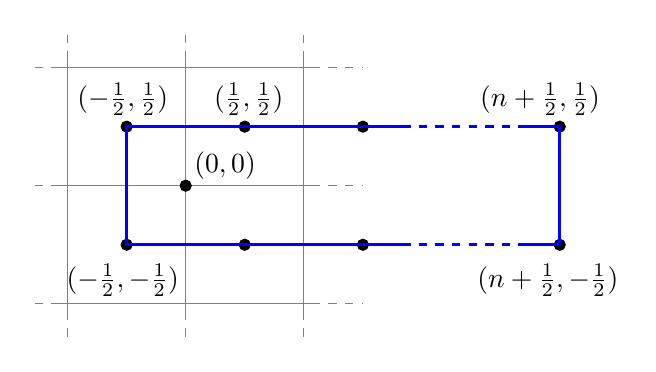
\begin{tikzpicture}
        \draw[gray] (-1.6, 1.5) -- (1.6, 1.5);
        \draw[gray] (-1.6, 0.0) -- (1.6, 0.0);
        \draw[gray] (-1.6, -1.5) -- (1.6, -1.5);
        
        \draw[gray] (-1.5, 1.6) -- (-1.5, -1.6);
        \draw[gray] (0.0, 1.6) -- (0.0, -1.6);
        \draw[gray] (1.5, 1.6) -- (1.5, -1.6);
        
        \draw[gray, dashed] (-1.5, -1.6) -- (-1.5, -2.0);
        \draw[gray, dashed] (0, -1.6) -- (0, -2.0);
        \draw[gray, dashed] (1.5, -1.6) -- (1.5, -2.0);
        
        \draw[gray, dashed] (-1.5, 1.6) -- (-1.5, 2.0);
        \draw[gray, dashed] (0, 1.6) -- (0, 2.0);
        \draw[gray, dashed] (1.5, 1.6) -- (1.5, 2.0);
        
        \draw[gray, dashed] (-1.6, 1.5) -- (-2.0, 1.5);
        \draw[gray, dashed] (-1.6, 0.0) -- (-2.0, 0.0);
        \draw[gray, dashed] (-1.6, -1.5) -- (-2.0, -1.5);
        
        \draw[gray, dashed] (1.6, 1.5) -- (2.25, 1.5);
        \draw[gray, dashed] (1.6, 0.0) -- (2.25, 0.0);
        \draw[gray, dashed] (1.6, -1.5) -- (2.25, -1.5);
        
        % Origin
        \node at (0.5, 0.25) {$(0, 0)$};
        \filldraw (0, 0) circle (2.0pt);
        
        % Dual
        \filldraw[black] (0.75, 0.75) circle (2pt);
        \filldraw[black] (0.75, -0.75) circle (2pt);
        \filldraw[black] (-0.75, 0.75) circle (2pt);
        \filldraw[black] (-0.75, -0.75) circle (2pt);
        
        \filldraw[black] (2.25, 0.75) circle(2pt);
        \filldraw[black] (2.25, -0.75) circle(2pt);
        
        \filldraw[black] (4.75, 0.75) circle(2pt);
        \filldraw[black] (4.75, -0.75) circle(2pt);
        
        \node at (0.8, 1.10) {$(\frac{1}{2}, \frac{1}{2})$};
        \node at (-0.8, 1.10) {$(-\frac{1}{2}, \frac{1}{2})$};
        \node at (-0.8, -1.20) {$(-\frac{1}{2}, -\frac{1}{2})$};
        \node at (4.5, 1.10) {$(n + \frac{1}{2}, \frac{1}{2})$};
        \node at (4.6, -1.20) {$(n + \frac{1}{2}, -\frac{1}{2})$};
        
        % Cycle
        \draw[blue, very thick] (4.25, -0.75) -- (4.75, -0.75) -- (4.75, 0.75) -- (4.25, 0.75);
        \draw[blue, very thick] (2.75, -0.75) -- (-0.75, -0.75) -- (-0.75, 0.75) -- (2.75, 0.75);
        \draw[blue, very thick, dashed] (2.75, -0.75) -- (4.25, -0.75);
        \draw[blue, very thick, dashed] (2.75, 0.75) -- (4.25, 0.75);
    \end{tikzpicture}
    \caption{The shortest cycle in $(\Z^2)^*$ passing by $(n + \frac{1}{2}, \frac{1}{2})$ and surrounding $O$}
    \label{fig:shortest_cycle_dual}
\end{figure}